\chapter{Vergleich}
Hier wird nun die Klassische Lösung für den Zwei-Spin-Fall mit der exakten quantenmechanischen Lösung verglichen.
\section{quantenmechanische Lösung}
Für die exakte quantenmechanische Lösung, wird der Hamiltonian diagonalisiert über die Basis:
\begin{align}
    \ket{1} &= \ket{\uparrow\uparrow}   \\
    \ket{2} &= \ket{\downarrow\downarrow} \\
    \ket{3} &= \frac{1}{\sqrt{2}N_1}\left[(\epsilon_1+1)\ket{\uparrow\downarrow} +(\epsilon_1-1)\ket{\downarrow\uparrow} \right]\\
    \ket{4} &= \frac{1}{\sqrt{2}N_2}\left[(\epsilon_2+1)\ket{\uparrow\downarrow} +(\epsilon_2-1)\ket{\downarrow\uparrow} \right]
\end{align}
mit $\epsilon_{1,2} = \frac{\alpha \pm \sqrt{b^2(1-z)^2+\alpha^2} }{b(1-z)} $ und $N_{i} = \sqrt{\epsilon_i^2 + 1}$. Die dazugehörigen Eigenenergien lauten:
\begin{align}
    E_1 &= b(1+z) + \frac{\alpha}{4}\\
    E_2 &= -b(1+z) + \frac{\alpha}{4}\\
    E_3 &= -\frac{\alpha}{4} + \frac{\sqrt{\alpha^2 + b^2(1-z)^2}}{2}\\
    E_4 &= -\frac{\alpha}{4} - \frac{\sqrt{\alpha^2 + b^2(1-z)^2}}{2}\\
\end{align}
\noindent Über den Zeitentwicklungsoperator und einem beliebigen Startzustand $\ket{\Psi_0}$, lässt sich die Spindynamik hinschreiben als:
\begin{align}
    \bra{\Psi}\hat{S}_i\ket{\Psi} &= \sum_{i,j}e^{i(E_i-E_j)t}\bra{i}\hat{S}_i\ket{j}\bra{j}\ket{\Psi_0}\bra{\Psi_0}\ket{i}
\end{align}
\section{exemplarischer Vergleich}
\begin{wrapfigure}{r}{0.4\textwidth}
    \centering
    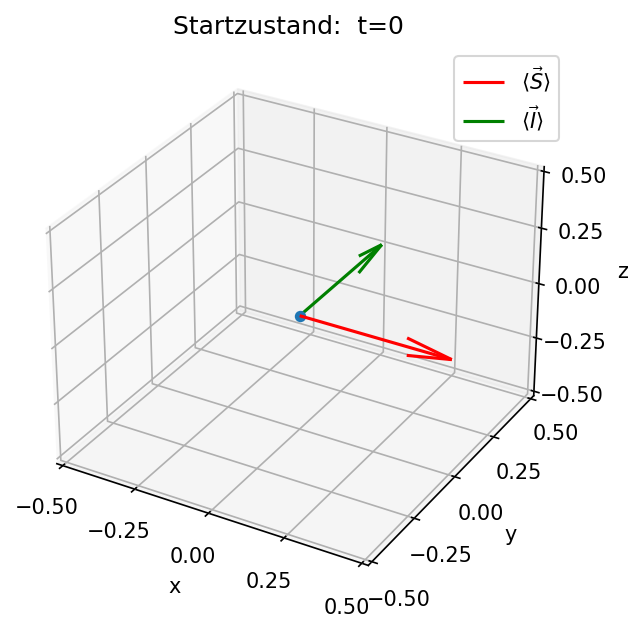
\includegraphics[width = 0.4\textwidth]{Abbildungen/Plot_Vektor_Start.png}
    \caption{gewählter Startzustand in einem 3D-Plot mit rotem Elektronenspinerwartungswert und grünem Kernspinerwartungswert als Vektoren dargestellt}
    \label{fig:Plots_Start}
\end{wrapfigure}
Es wird der Startzustand 
\begin{align}
    \ket{\Psi_0}=\ket{\uparrow\uparrow} + i\ket{\uparrow\downarrow} + \ket{\downarrow\uparrow} + i\ket{\downarrow\downarrow}
\end{align}
verwendet, welcher Äquivalent zu eine Elektronenspinerwartungswert entlang der X-Achse und orthogonal
dazu dem Kernspinerwartungswert entlang der Y-Achse, beide auf der X-Y-Ebene liegend wie in \autoref{fig:Plots_Start} zu sehen.
Unter all den möglichen Startzuständen gewählt, da dies ein sehr einfachen und anschaulichen Fall darstellt, da das Magnetfeld und beide Spinvektoren 
ein Dreibein bilden und gleich zu Beginn die Kopplungen unter einander durch die Orthogonalität am stärksten ist.


\begin{figure}[h]
    \centering
    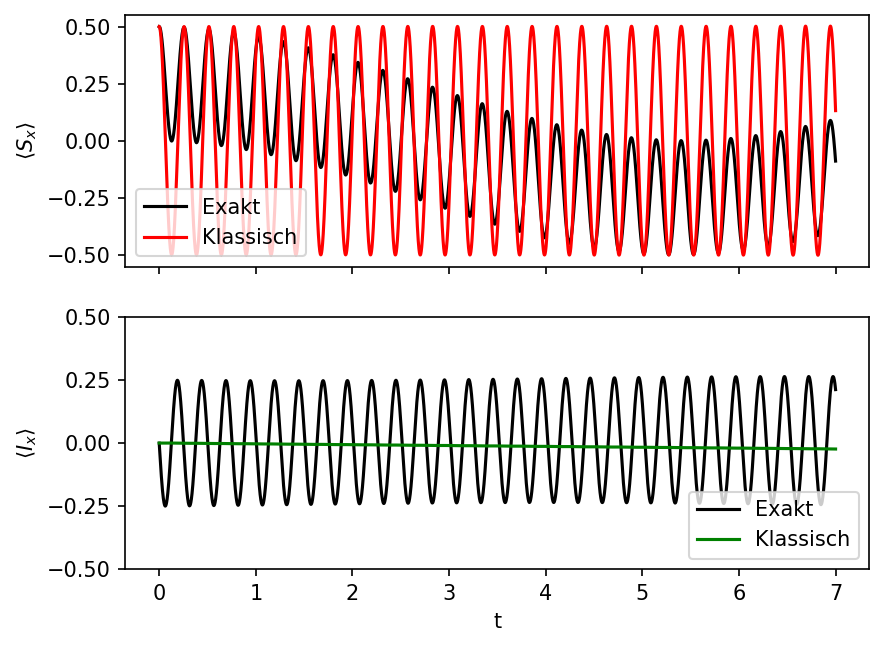
\includegraphics[width = 0.45\textwidth]{Abbildungen/Plot_Sx.png}
    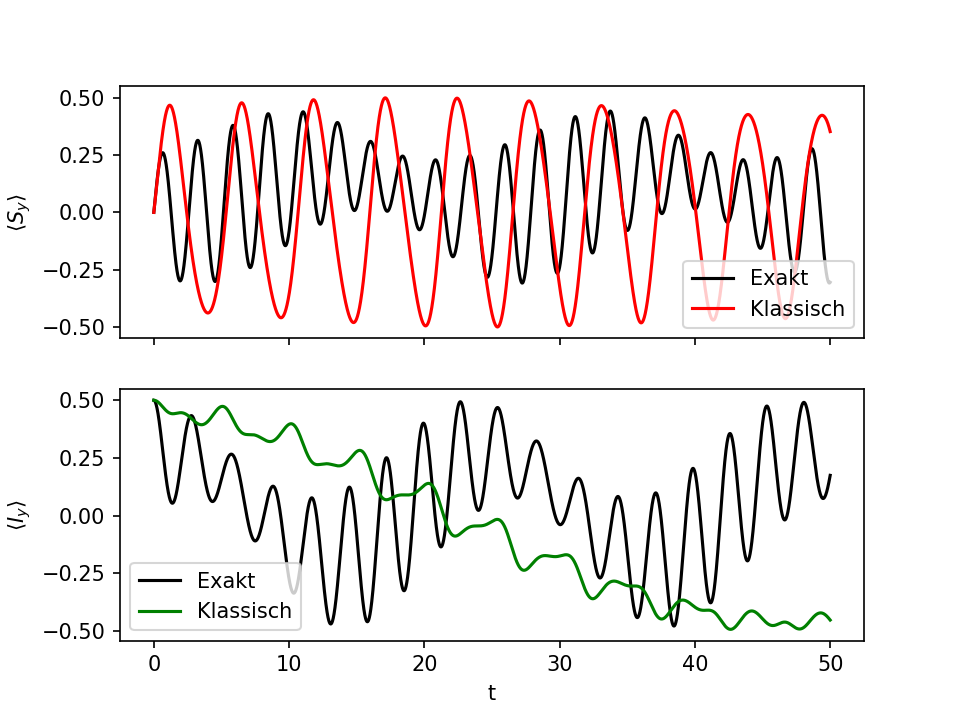
\includegraphics[width = 0.45\textwidth]{Abbildungen/Plot_Sy.png}
    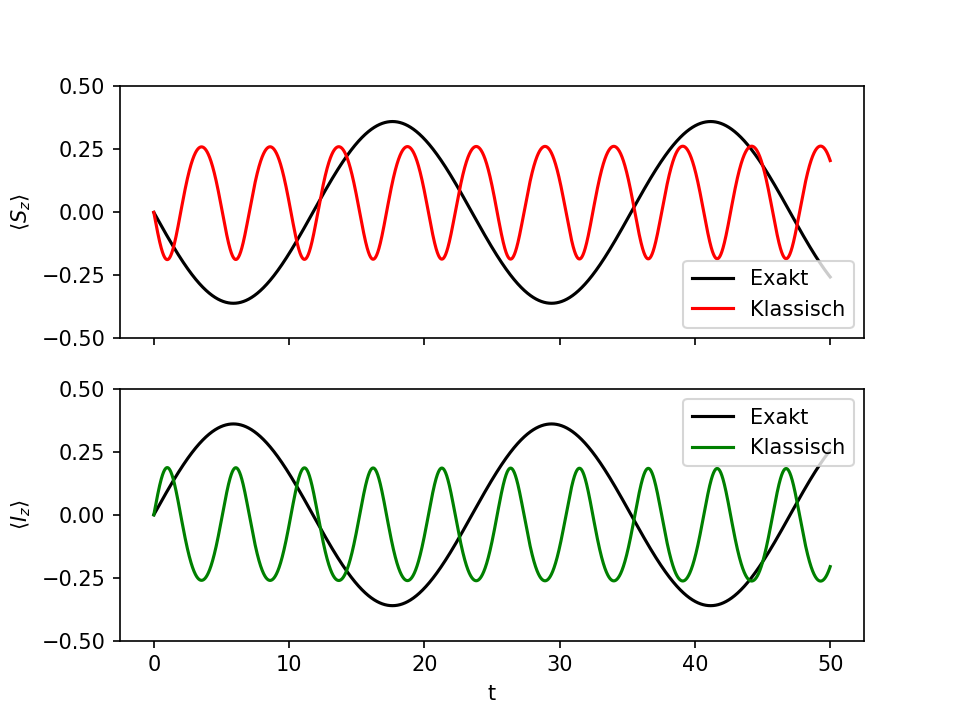
\includegraphics[width = 0.45\textwidth]{Abbildungen/Plot_Sz.png}
    \caption{Spin-Erwartungswerte des Elektronenspins S (Rot) und des Kernspins (Grün) und der jeweils exakten quantenmechanischen Lösung
    (Schwarz) gegen die Zeit t aufgetragen für die Parameter: ...}
    \label{fig:Plots_2D}
\end{figure}

\begin{figure}[h]
    \centering
    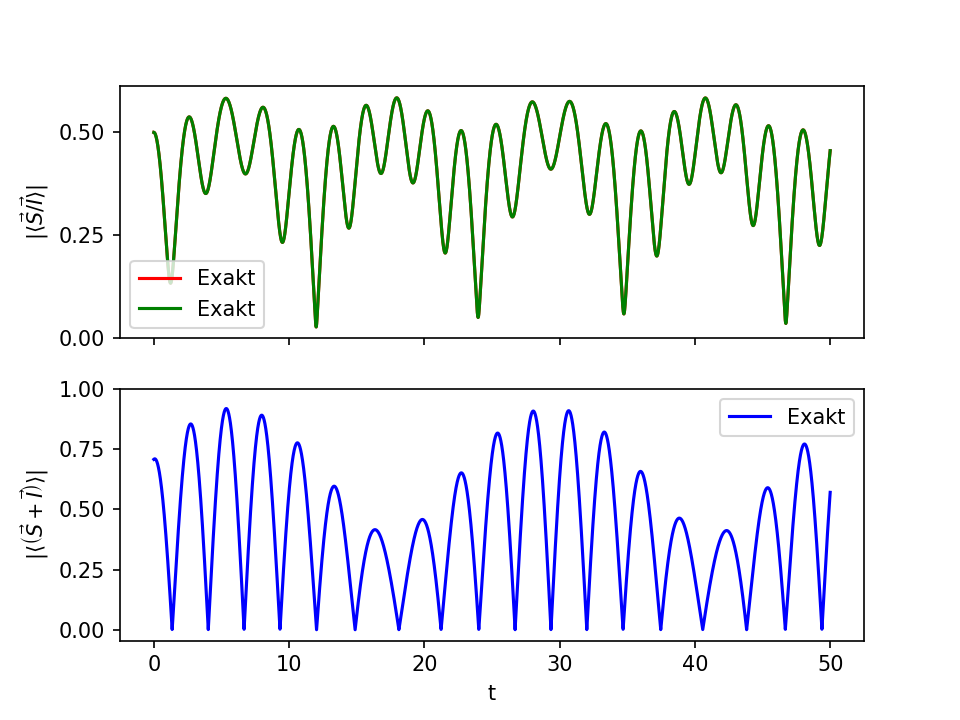
\includegraphics[width = 0.45\textwidth]{Abbildungen/Plot_Spin_length.png}
    \caption{oben: Spinlänge-Erwartungswert des Kernspin und Elektronenspin gegen die Zeit aufgetragen.
    unten: Spinlänge der addierten Spins gegen die Zeit aufgetragen}
    \label{fig:Plots_Spinlength}
\end{figure}


\begin{figure}[h!]
    \centering
    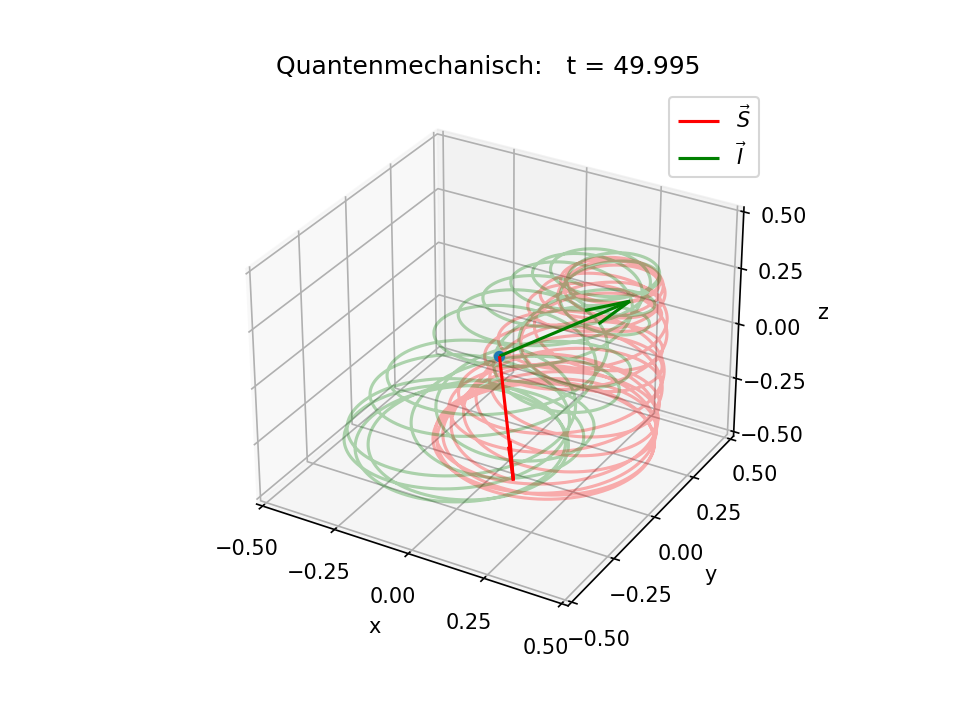
\includegraphics[width = 0.45\textwidth]{Abbildungen/Plot_Vektor_Quant.png}
    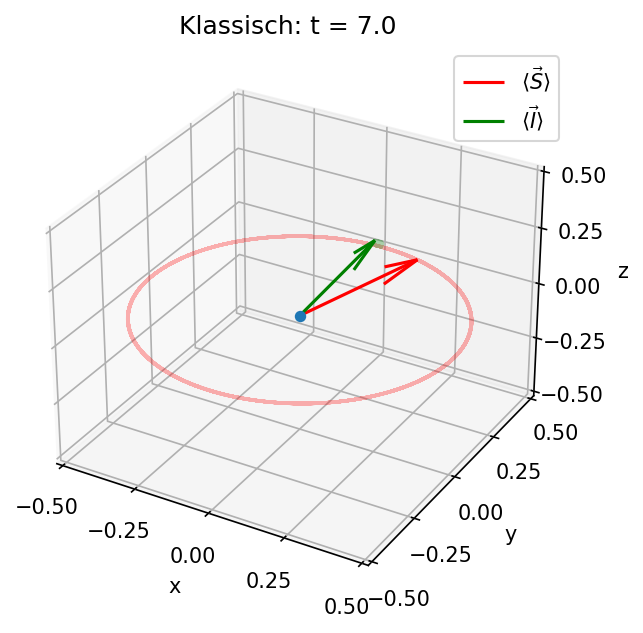
\includegraphics[width = 0.45\textwidth]{Abbildungen/Plot_Vektor_Klassisch.png}
    \caption{Spinerwartungswerte als Vektoren zum Endzeitpunkt des betrachten Zeitraums zum genannten Startzustand samt abgefahrener Spur der
    quantenmechanischen Lösung (Links) und der klassischen Lösung (Rechts)}
    \label{fig:Plots_3D}
\end{figure}


